\documentclass[a4paper, 12pt]{article}

\usepackage{underbrace}

\usepackage{graphicx}

\usepackage[left=1cm, right=1cm, top=2cm, bottom=2cm]{geometry}

\usepackage{animate} 

\usepackage[table]{xcolor}

\usepackage [russian]{babel}
\usepackage{amssymb,amsmath,latexsym,amsfonts,amsthm}

\renewcommand{\arraystretch}{1.1}

\usepackage{array}
\newcolumntype{P}[1]{>{\centering\arraybackslash}p{#1}}
\newcolumntype{M}[1]{>{\centering\arraybackslash}m{#1}}

\usepackage{hyperref}
\hypersetup{
    colorlinks=true,
    linkcolor=blue,
    filecolor=magenta,      
    urlcolor=cyan,
}

\begin{document}

\begin{center}
\Huge{\textbf{Mathematical model of self-focusing}}
\end{center}

We obtain the self-focusing equation in the approximation of a slowly varying amplitude to study the propagation of beams including multimedia -- annular beams with phase singularity on the optical axis.

\section{Obtaining a self-focusing equation}

The numerical simulation of optical vortex propagation is based on nonlinear wave equation, which could be obtained starting with Maxwell's system of equations:
\begin{equation}
\label{eqn:maxwell}
\left\{
\begin{aligned}
\nabla \times \mathbf{E}(\mathbf{r}, t) &= -\frac{\partial \mathbf{B}(\mathbf{r}, t)}{\partial t},\\
\nabla \times \mathbf{H}(\mathbf{r}, t) &= \mathbf{j}(\mathbf{r}, t) + \frac{\partial \mathbf{D}(\mathbf{r}, t)}{\partial t},\\[0.2cm]
\nabla \cdot \mathbf{D}(\mathbf{r}, t) &= \rho_f (\mathbf{r}, t) + \rho_b (\mathbf{r}, t), \\[0.3cm]
\nabla \cdot \mathbf{B}(\mathbf{r}, t) &= 0.
\end{aligned}
\right.
\end{equation}
where $\mathbf{E}(\mathbf{r}, t)$ и $\mathbf{D}(\mathbf{r}, t)$ -- electric field and induction, $\mathbf{H}(\mathbf{r}, t)$ и $\mathbf{B}(\mathbf{r}, t)$ -- magnetic field and induction, $\mathbf{\rho_f}(\mathbf{r}, t)$ и $\mathbf{\rho_b}(\mathbf{r}, t)$ -- density of free and bound electric charges. $\mathbf{j}(\mathbf{r}, t)$ -- conduction current density. The relationship of electric field and induction is given in the form:
\begin{equation}
\label{eqn:D}
\mathbf{D}(\mathbf{r}, t) = \varepsilon_0 \mathbf{E}(\mathbf{r}, t) + \mathbf{P}(\mathbf{r}, t)
\end{equation}
where $\mathbf{P}(\mathbf{r}, t)$ -- polarization, $c = \sqrt{1 / \varepsilon_0 \mu_0}$ -- light speed, $\varepsilon_0$ и $\mu_0$ -- dielectric and magnetic constants.

Considering medium is dielectric ($\mathbf{\rho_f}(\mathbf{r}, t) = 0$) and nonmagnetic ($\mathbf{B}(\mathbf{r}, t) = \mu_0 \mathbf{H}(\mathbf{r}, t)$) 
we get:
\begin{equation}
\label{eqn:prototype}
\Delta \mathbf{E}(\mathbf{r}, t) - \nabla (\nabla \cdot \mathbf{E}(\mathbf{r}, t)) =  \frac1{\varepsilon_0 c^2} \frac{\partial \mathbf{j}(\mathbf{r}, t)}{\partial t} + \frac1{c^2} \frac{\partial^2 \mathbf{E}(\mathbf{r}, t)}{\partial t^2} + \frac1{\varepsilon_0 c^2} \frac{\partial^2 \mathbf{P}(\mathbf{r}, t)}{\partial t^2},
\end{equation}
where $\mathbf{E}$ is electric field, $\mathbf{j}$ is current density and $\mathbf{P}$ is polarization, $c=1/\sqrt{\varepsilon_0 \mu_0}$. We examine each of equation \eqref{eqn:prototype} members one by one using several further approximations. 

Assuming paraxiality, that is transverse wave number is much smaller than longitudinal one, $k_\perp \ll k_z$, and linear polarization of the electric field $\mathbf{E}$, we can use method of slowly varying amplitude $\mathbf{E}$:
\begin{equation}
\mathbf{E}(\mathbf{r}, t) = \frac1{2}\mathbf{e} A(\mathbf{r}, t) \exp\{i (\omega_0 t - k_0 z)\} + \text{c.c.}
\end{equation}
where $A(\mathbf{r}, t)$ is a complex slowly varying amplitude, $\mathbf{e}$ is a unit vector.
Using dipole approximation ($\chi^{(i)}(\mathbf{r},t) = \chi^{(i)}(t)$) we can write ($\otimes$ means convolution) polarization as:
\begin{multline}
\label{eqn:polarizations}
\mathbf{P}(\mathbf{r}, t) = \mathbf{P}^{(1)}(\mathbf{r}, t) + \mathbf{P}^{(2)}(\mathbf{r}, t) + \mathbf{P}^{(3)}(\mathbf{r}, t) + ... = \varepsilon_0 \chi^{(1)}(t) \otimes \mathbf{E}(\mathbf{r}, t) +\\+ \varepsilon_0  \chi^{(2)}(t) \otimes \mathbf{E}(\mathbf{r}, t) \mathbf{E}(\mathbf{r}, t) + \varepsilon_0  \chi^{(3)}(t) \otimes \mathbf{E}(\mathbf{r}, t) \mathbf{E}(\mathbf{r}, t) \mathbf{E}(\mathbf{r}, t) + ...
\end{multline}
where $\chi^{(i)}(t)$ -- permittivity tensor of $i$-th order. We consider isotropic medium ($\mathbf{P}^{(2 m)}(\mathbf{r}, t)=0, \ m \in \mathbb{N}$). Each $(n+2)$-th term of the polarization series \eqref{eqn:polarizations} refers to $n$-th one as $\sim \bigl|I(\mathbf{r}, t) \bigr| \bigl/ \bigl|I_a \bigr|$, where $I_a \sim 5 \times 10^{16}$ W/cm$^2$ is atomic intensity. Peak intensity inside the filament is about $5 \times 10^{13}$ W/cm$^2$, so the ratio is of the order of $\sim 10^{-3}$. We can neglect nonlinearities of higher orders and write:
\begin{equation}
\mathbf{P}(\mathbf{r}, t) = \mathbf{P}^{(1)}(\mathbf{r}, t) + \mathbf{P}^{(3)}(\mathbf{r}, t).
\end{equation}
Therefore we will limit our consideration only to linear and cubic polarizations. Linear polarization can be written as
\begin{multline}
\mathbf{P}^{(1)}(\mathbf{r}, t) = \varepsilon_0 \chi^{(1)}(t) \otimes \mathbf{E}(\mathbf{r}, t) =
\varepsilon_0 \int\limits_{-\infty}^{+\infty} \chi^{(1)}(\tau) \mathbf{E}(\mathbf{r}, t - \tau) d\tau =\\= \frac1{2}\mathbf{e} \exp\{i (\omega_0 t  - k_0 z)\} \varepsilon_0 \int\limits_{-\infty}^{+\infty} \chi^{(1)}(\tau)  A(\mathbf{r}, t - \tau) \exp\{-i \omega_0 \tau \} d\tau.
\end{multline}
Using inverse Fourier transform of slowly varying electric field amplitude 
\begin{equation}
A(\mathbf{r}, t) = \frac1{2 \pi} \int\limits_{-\infty}^{+\infty} \tilde{A}(\mathbf{r}, \Omega) \exp \{ i \Omega t \} d \Omega,
\end{equation}
forward Fourier transform of electric susceptibility
\begin{equation}
\label{eqn:susceptibility_fourier}
\tilde{\chi}^{(1)}(\omega) = \int\limits_{-\infty}^{+\infty} \chi^{(1)}(t) \exp \{ -i \omega t \} dt
\end{equation}
and relation between susceptibility and wave vector $\tilde{\chi}^{(1)}(\omega) = k^2(\omega) c^2 / \omega^2 - 1$, we obtain
\begin{equation}
\mathbf{P}^{(1)}(\mathbf{r}, t) = \frac1{2}\mathbf{e} \exp\{i (\omega_0 t  - k_0 z)\} \varepsilon_0 c^2 \frac1{2 \pi} \int\limits_{-\infty}^{+\infty} \frac{k^2(\omega_0 + \Omega)}{\omega_0^2 + 2 \omega_0 \Omega + \Omega^2} \tilde{A}(\mathbf{r}, \Omega) \exp \{ i \Omega t \} d \Omega - \varepsilon_0 \mathbf{E}(\mathbf{r}, t),
\end{equation}
where $k(\omega) = \omega n(\omega)/ c$, $n(\omega)$ -- index of refraction. The linear part of the last term in equation \eqref{eqn:prototype} takes the form:
\begin{equation}
\label{eqn:p1_derivative}
\frac1{\varepsilon_0 c^2} \frac{\partial^2 \mathbf{P}^{(1)}(\mathbf{r}, t)}{\partial t^2} = -\frac1{2}\mathbf{e} \exp\{i (\omega_0 t  - k_0 z)\}   \frac1{2 \pi} \int\limits_{-\infty}^{+\infty} k^2(\omega_0 + \Omega) \tilde{A}(\mathbf{r}, \Omega) \exp \{ i \Omega t \} d \Omega - \frac1{c^2} \frac{\partial^2 \mathbf{E}(\mathbf{r}, t)}{\partial t^2}.
\end{equation}
The expression for cubic polarization consists of two terms related to the first and third harmonics:
\[
\mathbf{P}^{(3)}(\mathbf{r}, t) = \varepsilon_0  \chi^{(3)}(t) \otimes \mathbf{E}(\mathbf{r}, t) \mathbf{E}(\mathbf{r}, t) \mathbf{E}(\mathbf{r}, t) =
\]
\[= \frac1{8} \mathbf{e} \exp \{ i (3 \omega_0 t - 3 k_0 z) \}\varepsilon_0  \iiint \chi^{(3)}(\tau_1, \tau_2, \tau_3) A(\mathbf{r}, t - \tau_1)  A(\mathbf{r}, t - \tau_2) A(\mathbf{r}, t - \tau_3) \times 
\]
\[
 \times \exp\{-i \omega_0 (\tau_1 + \tau_2 + \tau_3) \} d\tau_1 d\tau_2 d \tau_3 + 
\]
\[
+ \frac{3}{8} \mathbf{e} \exp \{ i (\omega_0 t - k_0 z) \} \varepsilon_0  \iiint \chi^{(3)}(\tau_1, \tau_2, \tau_3) A(\mathbf{r}, t - \tau_1)  A(\mathbf{r}, t - \tau_2)  A^*(\mathbf{r}, t - \tau_3) \times 
\]
\begin{equation}
\times \exp\{-i \omega_0 (\tau_1 + \tau_2 - \tau_3) \} d\tau_1 d\tau_2 d \tau_3.
\end{equation}
Due to strong violation of wave synchronism, $\Delta k = 3 k (\omega_0) - k(3 \omega_0) \ne 0$, we neglect the third harmonic generation. Fourier transform of 3-th order electric susceptibility (similarly to \eqref{eqn:susceptibility_fourier}) and well-known relation between intensity and electric field amplitude  $I(\mathbf{r}, t) = c n_0 \varepsilon_0 |A(\mathbf{r}, t)|^2 \bigl/ 2$ yield
\begin{equation}
\mathbf{P}^{(3)}(\mathbf{r}, t) = \frac{3}{4} \mathbf{e} \exp \{ i (\omega_0 t - k_0 z) \} \varepsilon_0 \frac{\tilde{\chi}^{(3)}}{c n_0 \varepsilon_0} I(\mathbf{r}, t) A(\mathbf{r}, t).
\end{equation}
The second time derivative of nonlinear polarization in \eqref{eqn:prototype} takes the form
\begin{equation}
\label{eqn:p3_derivative}
\frac1{\varepsilon_0 c^2} \frac{\partial^2 \mathbf{P}^{(3)}(\mathbf{r}, t)}{\partial t^2} = -\frac1{2} \mathbf{e} \exp \{ i (\omega_0 t - k_0 z) \} \frac{2 k_0^2}{n_0} \hat{T}^2 \Delta n_k(\mathbf{r}, t) A(\mathbf{r}, t), 
\end{equation}
where
\begin{equation}
\hat{T} = 1 - \frac{i}{\omega_0} \frac{\partial}{\partial t}
\end{equation}
is the operator of wave-nonstationarity, which provides more accurate description of short pulse propagation compared to commonly used approximation of this operator by unit.

In case of instant response the nonlinear (Kerr) addition to the refractive index $\Delta n_k(\mathbf{r}, t) = n_2 I(\mathbf{r}, t)$, where $n_2 = 3 \tilde{\chi}^{(3)} \bigl/ 4 c n_0^2 \varepsilon_0$.

We will consider only self-focusing process without taking into account the ionization in the medium by a strong laser field, so $\mathbf{j}(\mathbf{r}, t)=0$

Substituting the expressions \eqref{eqn:p1_derivative}, \eqref{eqn:p3_derivative} to \eqref{eqn:prototype}, assuming $\nabla \cdot \mathbf{E}(\mathbf{r}, t) = 0$ and expanding the Laplace operator to transverse and longitudinal parts $\Delta = \Delta_\perp + \partial^2/\partial z^2$ we obtain nonlinear wave equation, which can be written in retarded time $t'=t-k_1 z$ and $z'=z$ coordinates as
\begin{multline}
\label{eqn:equation_without_dissipation}
\frac{\partial^2 A (\mathbf{r}, t', z')}{\partial z'^2} - 2 i k_0  \biggl( 1 - \frac{i k_1}{k_0} \frac{\partial }{\partial t'}  \biggr) \frac{\partial A (\mathbf{r}, t', z')}{\partial z'} + \Delta_{\perp} A (\mathbf{r}, t', z')= \\ =-\frac1{2 \pi} \int\limits_{-\infty}^{+\infty} \Bigl( k^2(\omega_0 + \Omega) - (k_0 + k_1 \Omega)^2 \Bigr) \tilde{A}(\mathbf{r}, \Omega, z') \exp \{ i \Omega t' \} d \Omega - \frac{2 k_0^2}{n_0} \hat{T}^2 \Delta n_k(\mathbf{r}, t') A(\mathbf{r}, t', z'),
\end{multline}
where $k_1 = dk / d\omega |_{\omega=\omega_0}$. We neglect the second derivative of the field $A$ on $z'$ due to slowly varying amplitude approximation, assume the factor $k_1/k_0$ in brackets approximately equals to $1/\omega_0$ and redesignate $t'$, $z'$ back to $t$, $z$. 

Since the original problem is limited to the consideration of spatial effects, it will be assumed that the pulses are long enough and will not take into account temporal effects, therefore, we equate the dispersion integral to zero and remove the wave-nonstationarity operator $\hat{T}$. Then we get:
\begin{equation}
\label{eqn:approx_final}
\frac{\partial^2 A (\mathbf{r}, z)}{\partial z^2} - 2 i k_0 \frac{\partial A (\mathbf{r}, z)}{\partial z} + \Delta_{\perp} A (\mathbf{r}, z)= - \frac{2 k_0^2}{n_0} n_2 I(\mathbf{r}, z) A(\mathbf{r}, z).
\end{equation}
We use the quasi-optical approximation assuming $| \partial^2 A(\mathbf{r}, z) / \partial z^2| \ll k_0 |\partial A(\mathbf{r},z) / \partial z|$ and get the final equation of 3D-beam self-focusing  propagating in cubic nonlinear media in approximation of slowly varying field amplitudes:
\begin{equation}
\label{eqn:final}
2 i k_0 \frac{\partial A (\mathbf{r}, z)}{\partial z} = \Delta_{\perp} A (\mathbf{r}, z) + \frac{2 k_0^2}{n_0} n_2 I(\mathbf{r}, z) A(\mathbf{r}, z),
\end{equation}
where $\mathbf{r}$ -- transversal radius-vector, $z$ -- evolutionary coordinate, $A(\mathbf{r},z)$ -- complex slowly varying amplitude of laser field, $k_0$ -- wave vector, $\Delta_\perp$ -- transversal laplacian, $n_0$ -- linear refractive index, $n_2$ -- cubic nonlinear refractive index, $I(\mathbf{r},z)$ -- intensity of laser field. 

\section{Wave equation and initial conditions}

The amplitude of the laser field $A(\mathbf{r},z)$ depends on the radius vector $\mathbf{r}$, which in the general case can be represented as two transverse spatial coordinates $x$ and $y$. However, there is also an axisymmetric approximation according to which the field $A(\mathbf{r},z)$ does not depend on the polar angle $\varphi$ and therefore the radius vector $\mathbf{r}$ can be replaced by a scalar value $r$. Wave equation and initial conditions in these two cases will look different.

\subsection{$\mathbf{r}\longrightarrow(x,y)$}

Wave equation \eqref{eqn:final} takes the form:
\begin{equation}
2 i k_0 \frac{\partial A (x, y, z)}{\partial z} = \biggl[ \frac{\partial^2}{\partial x^2} + \frac{\partial^2}{\partial y^2} \biggr] A (x, y, z) + \frac{2 k_0^2}{n_0} n_2 I(x, y, z) A(x, y, z)
\end{equation}
The general form of initial conditions is
\begin{equation}
\label{eqn:initial_xy}
A(x,y, z = 0) = \biggl(1 + C \xi(x,y)\biggr)A_0 \biggl(\frac{x^2}{x_0^2}+\frac{y^2}{y_0^2}\biggr)^{M/2}\exp\biggl\{-\frac1{2}\biggl(\frac{x^2}{x_0^2}+\frac{y^2}{y_0^2}\biggr)\biggr\}\exp\biggl\{i m \varphi(x,y)\biggr\},
\end{equation}
where $x$ and $y$ -- transversal coordinates, $x_0$ and $y_0$ -- spatial parameters along corresponding coordinates, $M$ -- parameter describing the inner form of the beam ring, $m$ -- topological charge, $\varphi=\arctan{x/y}$, $\xi=\xi(\mathbb{E}, \sigma, r_{corr})$ -- gaussian noise with expectation $\mathbb{E}$, dispersion $\sigma^2$ and correlation radius $r_{corr}$. Vortex phase is defined as $\theta(x,y) = m \varphi(x,y)$.


\subsection{$\mathbf{r}\longrightarrow r$}

Wave equation \eqref{eqn:final} takes the form:
\begin{equation}
2 i k_0 \frac{\partial A (r, z)}{\partial z} = \biggl[ \frac{\partial^2}{\partial r^2} + \frac1{r}\frac{\partial}{\partial r} - \frac{m^2}{r^2} \biggr] A (r, z) + \frac{2 k_0^2}{n_0} n_2 I(r, z) A(r, z)
\end{equation}
The general form of initial conditions is
\begin{equation}
A(r,z=0) = A_0 \biggl( \frac{r}{r_0} \biggr)^M \exp \biggl\{ -\frac{r^2}{2r_0^2} \biggr\}
\end{equation}

\subsection{2D beam}

If we consider a two-dimensional beam, i.e. beam with one transverse spatial coordinate $x$, then the self-focusing equation \eqref{eqn:final} for it will be:
\begin{equation}
2 i k_0 \frac{\partial A (x, z)}{\partial z} = \frac{\partial^2 A (x, z)}{\partial x^2} + \frac{2 k_0^2}{n_0} n_2 I(x, z) A(x, z)
\end{equation}
Under the conditions of the one transverse coordinate $x$ presence, the assignment of any phase front is impossible; therefore, the initial condition has the general form of a collimated beam:
\begin{equation}
A(x,z=0) = A_0 \biggl( \frac{x}{x_0} \biggr)^M \exp \biggl\{ -\frac{x^2}{2x_0^2} \biggr\}
\end{equation}

\subsection{Types of initial conditions}

Depending on the values $M$ and $m$ ($M, m \in \mathbb{N}$), the initial conditions can take different forms:
\begin{itemize}
\item \textbf{Gauss ($M=m=0$)} 
\item \textbf{Ring ($M>0$, $m=0$)} 
\item \textbf{Vortex ($M>0$, $m>0$)}
\end{itemize}
Examples:
\begin{center}
\begin{tabular}{M{1.5cm}M{5cm}M{5cm}M{5cm}}
\ & \cellcolor{gray!25}\textbf{Gauss ($M=m=0$)} & \cellcolor{gray!25}\textbf{Ring ($M=1$, $m=0$)} & \cellcolor{gray!25}\textbf{Ring ($M=2$, $m=0$)} \\
\cellcolor{gray!25} $\mathbf{I(x,y)}$ &
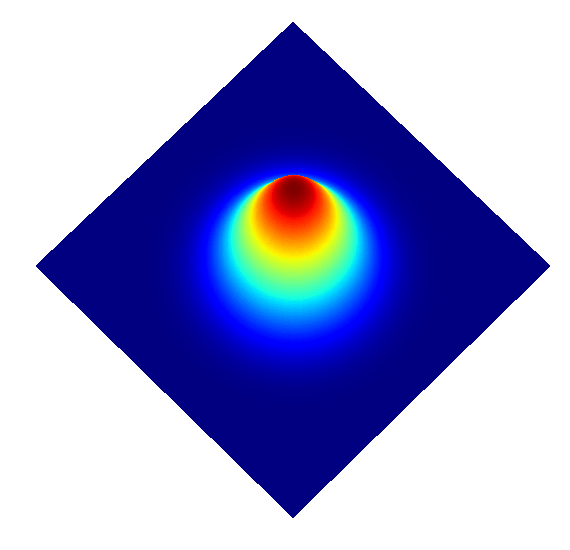
\includegraphics[width=\linewidth]{../resources/intensity_M=0.png} & 
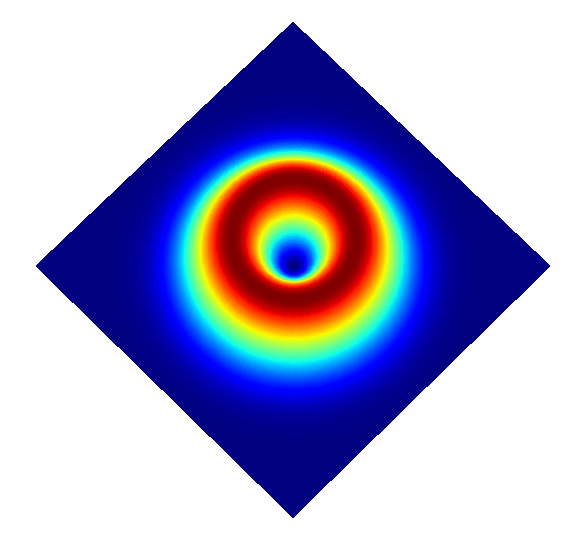
\includegraphics[width=\linewidth]{../resources/intensity_M=1.png} & 
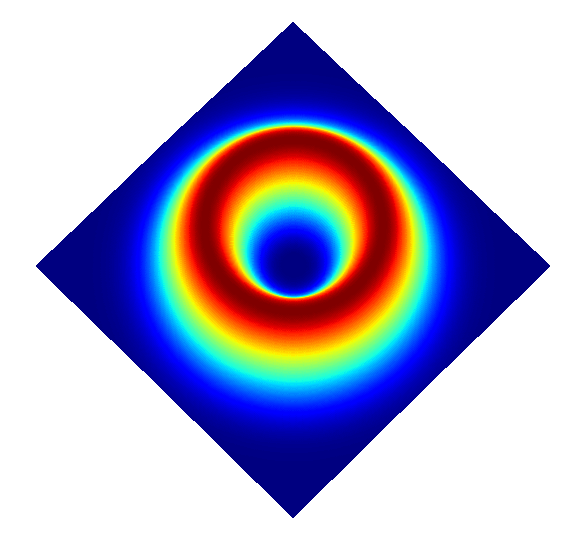
\includegraphics[width=\linewidth]{../resources/intensity_M=2.png}\\
\end{tabular}
\end{center}

\begin{center}
\begin{tabular}{M{1.5cm}M{5cm}M{5cm}M{5cm}}
\ & \cellcolor{gray!25}\textbf{Vortex ($M=1$, $m=1$)} & \cellcolor{gray!25}\textbf{Vortex ($M=2$, $m=2$)} & \cellcolor{gray!25}\textbf{Vortex ($M=3$, $m=3$)} \tabularnewline
\cellcolor{gray!25}$\mathbf{I(x,y)}$ &
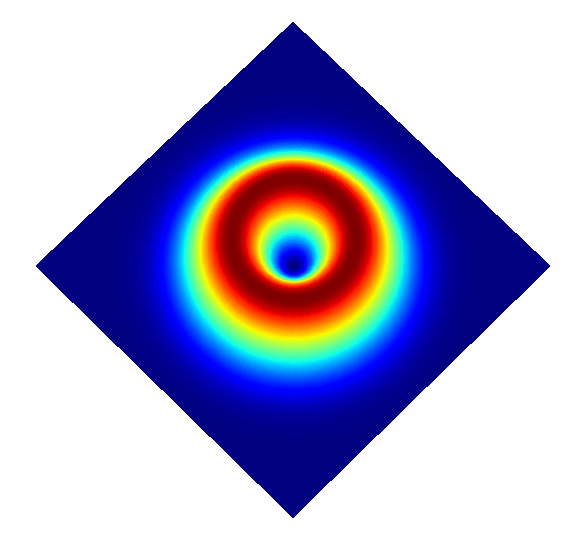
\includegraphics[width=\linewidth]{../resources/intensity_M=1.png} & 
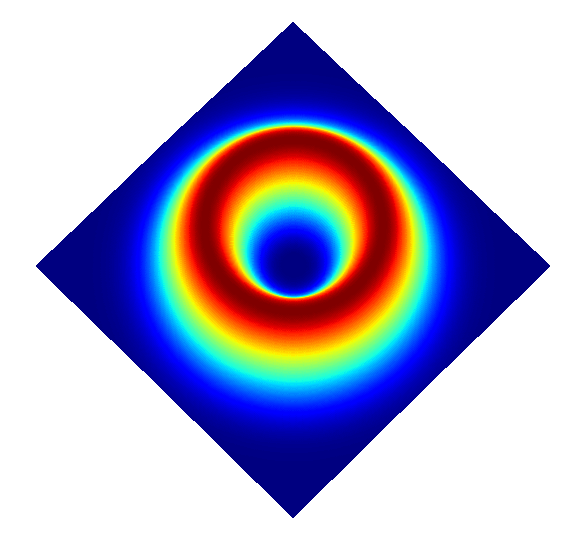
\includegraphics[width=\linewidth]{../resources/intensity_M=2.png} & 
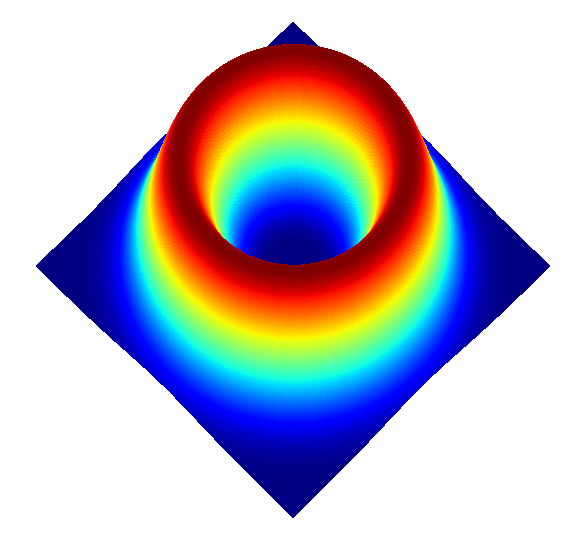
\includegraphics[width=\linewidth]{../resources/intensity_M=3.png} \\
\cellcolor{gray!25}$\mathbf{\theta(x,y)}$ & \ & \\
%\animategraphics[width=\linewidth, loop,controls=play]{180}{../resources/m=1_large/%images/}{0000}{0179} & 
%\animategraphics[width=\linewidth, loop,controls=play]{180}{../resources/m=2_large/%images/}{0000}{0179} & 
%\animategraphics[width=\linewidth, loop,controls=play]{180}{../resources/m=3_large/%images/}{0000}{0179}  \\
\end{tabular}
\end{center}
It should be noted that both the amplitude and phase profiles can be changed by the gaussian noise component.

\section{Numerical solution}

The nonlinear equation for the self-focusing of a laser beam \eqref{eqn:final} was solved by splitting into physical factors, according to which the initial equation is divided into a system of several equations, in which the solution of the $i$-th equation is the initial condition for $(i+1)$:
\begin{equation}
\left\{
\label{eqn:system}
\begin{split}
    2 i k_0  \frac{\partial A(\mathbf{r},z) }{\partial z}  &= \underbrace{\Delta_\perp A(\mathbf{r},z),}_{\textcolor{red}{\text{\small{diffraction}}}} \\
    2 i k_0  \frac{\partial A(\mathbf{r},z) }{\partial z} &= \underbrace{\frac{2 k_0^2}{n_0} n_2 I(\mathbf{r},z) A(\mathbf{r},z).}_{\substack{\text{\textcolor{red}{\small{Kerr}}}\\\text{\textcolor{red}{\small{nonlinearity}}}}}
\end{split}
\right.
\end{equation}

\subsection{Diffraction}
The solution of the beam diffraction equation differs depending on the approximation used.

\subsubsection{$\mathbf{r}\longrightarrow(x,y)$}

The diffraction equation in general case looks like:
\begin{equation}
\label{eqn:diffraction_xy}
2 i k_0 \frac{\partial A (x, y, z)}{\partial z} = \biggl[ \frac{\partial^2}{\partial x^2} + \frac{\partial^2}{\partial y^2} \biggr] A (x, y, z)
\end{equation}
We use the forward Fourier transform for turning to the spatial spectrum:
\begin{equation}
\label{eqn:fourier_xy}
A(x,y,z) = \frac1{\sqrt{2 \pi}}\iint\limits_{-\infty \quad}^{\quad+\infty} \tilde{A}(k_x, k_y, z) \exp \Bigl\{ i (k_x x + k_y y) \Bigr\} dk_x dk_y
\end{equation}
After substituting \eqref{eqn:fourier_xy} to \eqref{eqn:diffraction_xy}, we get:
\begin{equation}
2 i k_0 \frac{\partial \tilde{A} (k_x, k_y, z)}{\partial z} = -(k_x^2 + k_y^2) \tilde{A}(k_x, k_y, z)
\end{equation}
Finally we make up the problem of Cauchy
\begin{equation}
\label{eqn:diffraction_xy_cauchy}
\left\{
\begin{aligned}
\frac{\partial \tilde{A} (k_x, k_y, z)}{\partial z} &= R_{diff} \tilde{A} (k_x, k_y, z),\\
\tilde{A}(k_x, k_y, 0) &= \tilde{A}_0
\end{aligned}
\right.
\end{equation}
where
\begin{equation}
R_{diff} = i\frac{k_x^2 + k_y^2}{2 k_0}.
\end{equation}
The analytical solution for \eqref{eqn:diffraction_xy_cauchy} is
\begin{equation}
\tilde{A} = \tilde{A_0} \exp\{R_{diff} z\}.
\end{equation}
After introducing the following grids:
\begin{itemize}
\item $x\longrightarrow x_i, \ h_x = x_{i+1} - x_{i} = \text{const}, \ i = \overline{0, n_x-2}$
\item $k_x\longrightarrow k_{x_i}, \ h_{k_x} = k_{x_{i+1}} - k_{x_{i}} = \text{const}, \ i = \overline{0, n_x-2}$
\item $y\longrightarrow y_j, \ h_y = y_{j+1} - y_{j} = \text{const}, \ j = \overline{0, n_y-2}$
\item $k_y\longrightarrow k_{x_y}, \ h_{k_j} = k_{y_{j+1}} - k_{y_{j}} = \text{const}, \ j = \overline{0, n_y-2}$
\item $z\longrightarrow z_n, \ h_z = z_{n+1} - z_{n} \ne \text{const}, \ n = \overline{0, n_z-2}$
\item $\tilde{A} \longrightarrow \tilde{A}^n_{i, j}$
\end{itemize}
Knowing spectrum $\tilde{A}^n_{i,j}$ on $n$-th step on $z$, we get $\tilde{A}^{n+1}_{i,j}$:
\begin{equation}
\tilde{A}^{n+1}_{i,j} = \tilde{A}^n_{i,j} \exp\{R_{diff} h_z \}
\end{equation}

\subsubsection{$\mathbf{r}\longrightarrow r$}
In axisymmetric approximation diffraction equation looks like:
\begin{equation}
\label{eqn:diffraction_r}
2 i k_0 \frac{\partial A (r, z)}{\partial z} = \biggl[ \frac{\partial^2}{\partial r^2} + \frac1{r}\frac{\partial}{\partial r} - \frac{m^2}{r^2} \biggr] A(r,z)
\end{equation}
The numerical solution of the equation \eqref{eqn:diffraction_r} is associated with a grid approximation of the complex field for each of the coordinates, so we introduce the following grids:
\begin{itemize}
\item $r\longrightarrow r_k, \ h_r = r_{k+1} - r_{k} = \text{const}, \ k = \overline{0, n_r-2}$
\item $z\longrightarrow z_n, \ h_z = z_{n+1} - z_{n} \ne \text{const}, \ n = \overline{0, n_z-2}$
\item $A \longrightarrow A^n_{k, s}$
\end{itemize}

We use the Crank-Nicolson method with a central difference approximation of the derivatives:
\begin{equation}
\label{eqn:nikolson1}
\frac{\partial A}{\partial z} \longrightarrow \frac{\tilde{A}_k^{n+1} - A_k^{n}}{h_z}
\end{equation}
\begin{equation}
\label{eqn:nikolson2}
\frac{\partial^2 \tilde{A}}{\partial r^2} \longrightarrow \frac1{2} \biggl( \frac{\tilde{A}_{k+1}^{n+1} - 2 A_k^{n+1} + A_{k-1}^{n+1}}{h_r^2} \biggr) +
\frac1{2} \biggl( \frac{A_{k+1}^{n} - 2 A_k^{n} + A_{k-1}^{n}}{h_r^2} \biggl)
\end{equation}
\begin{equation}
\label{eqn:nikolson3}
\frac{\partial A}{\partial r} \longrightarrow \frac1{2} \biggl( \frac{A_{k+1}^{n+1} - A_{k-1}^{n+1}}{2h_r} \biggr) +
\frac1{2} \biggl( \frac{A_{k+1}^{n} - A_{k-1}^{n}}{2h_r} \biggl)
\end{equation}
Note that the order of approximation of the numerical scheme is $ O (h_r ^ 2, h_z ^ 2) $. Taking into account the expressions \eqref{eqn:nikolson1} - \eqref{eqn:nikolson3}, we write:
\begin{multline}
A_{k+1}^{n+1} \biggl( \frac1{2h_r^2} + \frac1{4 r_k h_r} \biggr) + A_{k}^{n+1} \biggl( -\frac{2 i k_0 \hat{T}_\Omega}{h_z} - \frac1{h_r^2} - \frac{m^2}{r_k^2}\biggr) + A_{k-1}^{n+1} \biggl(  \frac1{2h_r^2} - \frac1{4 r_k h_r} \biggr) =\\= A_{k+1}^{n} \biggl( -\frac1{2h_r^2} - \frac1{4 r_k h_r} \biggr) + A_{k}^{n} \biggl( -\frac{2 i k_0 \hat{T}_\Omega}{h_z} + \frac1{h_r^2} \biggr) + A_{k-1}^{n} \biggl( -\frac1{2h_r^2} + \frac1{4 r_k h_r} \biggr)
\end{multline}
The final expression for the grid approximation:
\begin{gather}
\alpha_kA_{k+1}^{n+1} - \beta_k A_{k}^{n+1} + \gamma_k A_{k-1}^{n+1} = -\delta_k\\
\alpha_k = \frac1{2h_r^2} + \frac1{4 r_k h_r}\\
\beta_k = \frac1{h_r^2} + \frac{2 i k_0 \hat{T}_\Omega}{h_z} + \frac{m^2}{r_k^2}\\
\gamma_k = \frac1{2h_r^2} - \frac1{4 r_k h_r}\\
\delta_k = \alpha_kA_{k+1}^{n} - \biggl(\beta^{*}_k - \frac{m^2}{r^2_k} \biggr) A_{k}^{n} + \gamma_k A_{k-1}^{n}
\end{gather}
General form of the boundary conditions:
\begin{gather}
A_0 = \kappa_{left} A_1 + \mu_{left}\\
A_{N_r-1} = \kappa_{right} A_{N_r-2} + \mu_{right}
\end{gather}
We represent the grid approximation taking into account the boundary conditions in the form of a matrix:
\begin{equation}
\label{eqn:3diagonal_maxtrix}
\begin{pmatrix}
1 & -\kappa_{left} & 0 & \dots & \dots & \dots & \dots\\
\gamma_1 & -\beta_1 & \alpha_1 & 0 & \dots & \dots & \dots\\
0 & \gamma_2 & -\beta_2 & \alpha_2 & 0 & \dots & \dots\\
\hdotsfor{7}\\
\hdotsfor{7}\\
\dots &\dots & 0 & \gamma_{N_r-3} & -\beta_{N_r-3} & \alpha_{N_r-3} & 0\\
\dots & \dots &\dots & 0 & \gamma_{N_r-2} & -\beta_{N_r-2} & \alpha_{N_r-2}\\
\dots &\dots &\dots &\dots & 0 & -\kappa_{right} & 1\\
\end{pmatrix}
\begin{pmatrix}
A_0 \\
A_1 \\
A_2 \\
\dots \\
\dots \\
A_{N_r-3} \\
A_{N_r-2} \\
A_{N_r-1}
\end{pmatrix}
=
\begin{pmatrix}
\mu_{left} \\
-\delta_1\\
-\delta_2\\
\dots \\
\dots \\
-\delta_{N_r-3}\\
-\delta_{N_r-2}\\
\mu_{right}
\end{pmatrix}
\end{equation}
The system of equations with the tridiagonal matrix \eqref{eqn:3diagonal_maxtrix} was solved by the sweep method.

\subsection{2D beam}

The diffraction in a two-dimensional beam is taken into account in the same way as in an axisymmetric one -- using the sweep method, but consideration of a two-dimensional beam simplifies the calculations for the final expression in the grid approximation:
\begin{gather}
\alpha_kA_{k+1}^{n+1} - \beta_k A_{k}^{n+1} + \gamma_k A_{k-1}^{n+1} = -\delta_k\\
\alpha_k = \frac1{2h_x^2}\\
\beta_k = \frac1{h_x^2} + \frac{2 i k_0 \hat{T}_\Omega}{h_z}\\
\gamma_k = \frac1{2h_x^2}\\
\delta_k = \alpha_kA_{k+1}^{n} - \beta^{*}_k A_{k}^{n} + \gamma_k A_{k-1}^{n}
\end{gather}



\subsection{Kerr nonlinearity}

The influence of the Kerr nonlinearity takes into account equally regardless of the dimension of the problem being solved. The equation describing Kerr effect takes the form:
\begin{equation}
2 i k_0  \frac{\partial A(\mathbf{r},z) }{\partial z} = \frac{2 k_0^2}{n_0} n_2 I(\mathbf{r},z) A(\mathbf{r},z)
\end{equation}
We make up the problem of Cauchy:
\begin{equation}
\label{eqn:diffraction_xy_cauchy}
\left\{
\begin{aligned}
 \frac{\partial A(\mathbf{r},z) }{\partial z} &= R_{kerr} A(\mathbf{r},z),\\
A(\mathbf{r}, 0) &= A_0
\end{aligned}
\right.
\end{equation}
where
\begin{equation}
R_{kerr} = -i\frac{k_0 n_2 I(\mathbf{r},z)}{n_0}
\end{equation}
Depending on the approximation, we introduce grids on the corresponding coordinates and get the solution in the form:
\begin{equation}
A^{n+1} = A^n \exp\{R_{kerr} h_z \}
\end{equation}



\section{Gaussian noise generation}

The laser beam propagation in reality is always accompanied by noise. Simulation of self-focusing in coordinates $x$ and $y$ allows to take into account the noise component, for example, in approximation of Gaussian complex noise $\xi(x,y)$ \eqref{eqn:initial_xy}. Gaussian noise with a predetermined dispersion $\sigma^2$ and correlation radius $r_{corr}$ can be generated according to the following algorithm:

\begin{itemize}
\item Generate a complex noise field array with shape of ($n_x$, $n_y$), the real and imaginary parts of which are evenly distributed in the range of $[-\sqrt{3}, +\sqrt{3}]$.
\item Multiply the real and imaginary part by the Gaussian envelope of the form:
\begin{equation}
G(i,j)= r_{corr}^* \sqrt{\pi \sigma^2} \exp \biggl\{ -\frac{(\pi r_{corr}^*)^2}{2} \biggl((i-0.5 n_x)^2 + (j-0.5 n_y)^2 \biggr) \biggr\}
\end{equation}
where $r_{corr}^*$ -- the number of grid nodes in $r_{corr}$.
\item Make inverse discrete Fourier transform and normalize the result array, if necessary.
\end{itemize}


\end{document}